\begin{figure}[!h]
	\centering
	\subbottom[example buildings\label{fig:egbui0}]{
		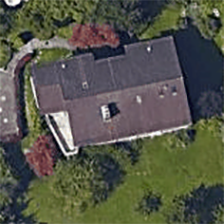
\includegraphics[width=\figfigfigfig\textwidth]{4-02-0.png}
		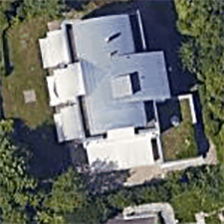
\includegraphics[width=\figfigfigfig\textwidth]{4-02-1.png}
		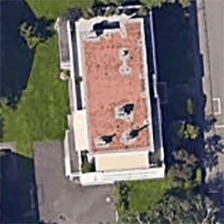
\includegraphics[width=\figfigfigfig\textwidth]{4-02-2.png}
		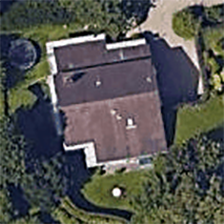
\includegraphics[width=\figfigfigfig\textwidth]{4-02-3.png}
	}
	\subbottom[example buildings with polygon outlines\label{fig:egbui1}]{
		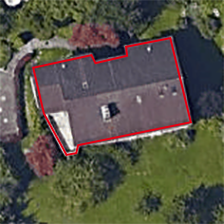
\includegraphics[width=\figfigfigfig\textwidth]{4-02-4.png}
		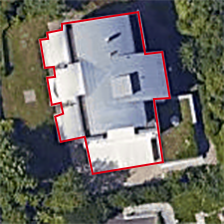
\includegraphics[width=\figfigfigfig\textwidth]{4-02-5.png}
		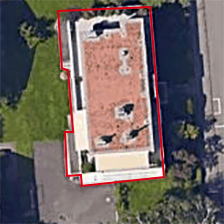
\includegraphics[width=\figfigfigfig\textwidth]{4-02-6.png}
		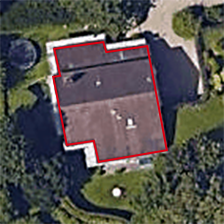
\includegraphics[width=\figfigfigfig\textwidth]{4-02-7.png}
	}
    \caption[Example buildings in Zurich for PolygonRNN training]{Example buildings in Zurich for PolygonRNN training. Images in (a) are the aerial images obtained by Google Static Maps API. (b) is (a) covered by the corresponding polygon outline, which is visualized based on the ground truth.}
	\label{fig:egbui}
\end{figure}